% !TeX root = ../main.tex
% Add the above to each chapter to make compiling the PDF easier in some editors.

\chapter{Background}\label{chapter:background}

Understanding the LAIK library as well as Inter Process Communication is fundamental for understanding the design of our shared memory backends. 
This chapter is divided into two parts. 
In the first, we will briefly introduce the fundamentals of LAIK, with particular emphasis on the topics of action sequences, the backend interface and data storage in LAIK. 
In the second part we will cover the necessary fundamentals of inter process communication, especially shared memory and semaphores.

\section{LAIK}

LAIK, which stands for \glqq Leichtgewichtige AnwendungsIntegriete Datenhaltungskomponente\grqq, is a library for data management in the HPC environment. 
Created out of the need for higher flexibility in regard to scheduling and fault tolerance strategies, LAIK provides support for distributing data across parallel applications by controlling the data and its partitioning. 
The goal of LAIK is to provide fault tolerance mechanisms and load balancing for HPC applications in the most lightweight and performant way possible \cite{laik-paper}. 
As shown in \autoref{fig:laik-layers}, LAIK sits between the application and the library used for communication.

\begin{figure}[h]
	\centering
	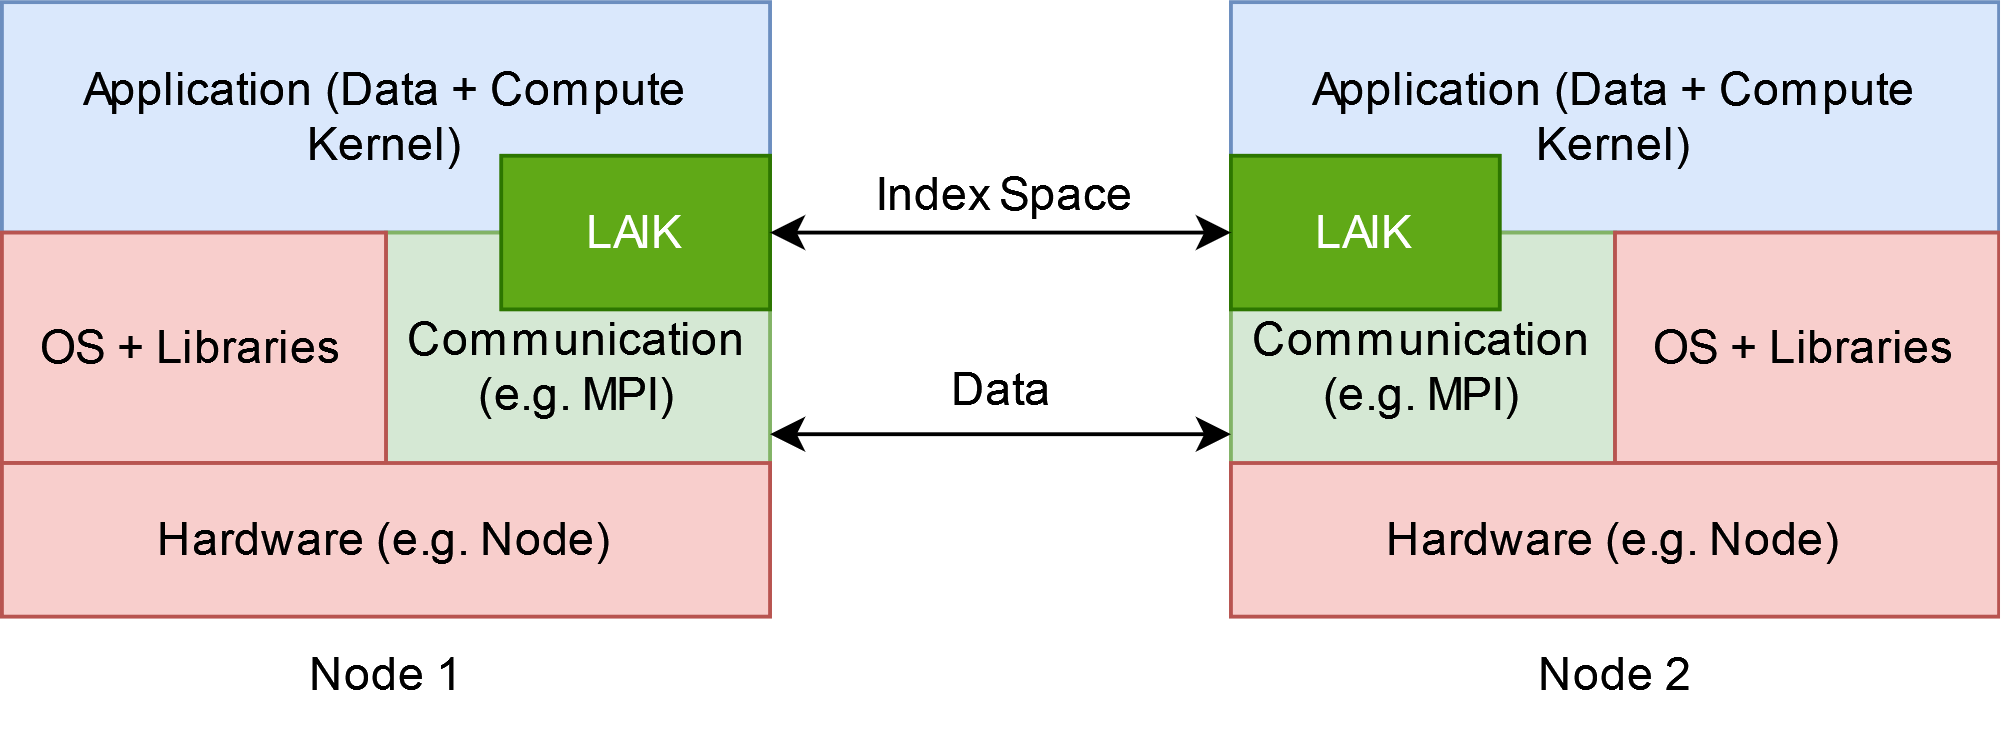
\includegraphics[width=0.75\columnwidth]{figures/laik-layers.png}
	\caption{LAIK and communication backend\cite{laik-paper}}
	\label{fig:laik-layers}
\end{figure}

\subsection{Action Sequences}

Action sequences are lists of actions which provide the information a node needs to execute a specific chain of actions. 
Actions are the atomic unit of execution in LAIK, they are predefined procedures which contain the necessary information for their own execution. 
LAIK creates action sequences based on the applications needs. 
After a sequence is created it can be optimised with the method \code{prepare()} before it is executed. 
When an action sequence is executed, the corresponding backend performs every action of the sequence in the set order. 
Action sequences can be executed multiple times. 
When an action sequence is not needed any more, it can be deleted by calling \code{cleanup()}.

\subsection{Backend Interface}

In LAIK backends are used to execute the data migration. 
As per its specification, LAIK supports different communication libraries to execute the data migration via a backend interface\cite{laik-paper}. 
When executing a LAIK application, the backend can be chosen by setting the environment variable \code{LAIK\_BACKEND} to the desired backend. Application programmers are able to implement new backends to use their desired communication library for LAIKs data migration \cite{laik-paper}.

\begin{figure}[htpb]
	\centering
	\begin{tabular}{c}
		\begin{lstlisting}[language=C++]
			struct _Laik_Backend {
				char* name;
				void (*finalize)(Laik_Instance*);
				void (*prepare)(Laik_ActionSeq*);
				void (*cleanup)(Laik_ActionSeq*);
				void (*exec)(Laik_ActionSeq*);
				void (*updateGroup)(Laik_Group*);
				void (*sync)(Laik_KVStore* kvs);
				bool (*log_action)(Laik_Action* a);
				void (*make_progress)();
				Laik_Group* (*resize)(Laik_ResizeRequests*);
				void (*finish_resize)();
			};
		\end{lstlisting}
	\end{tabular}
	\caption[LAIK-Backend struct]{A shortened version of the Laik\_Backend struct.}
	\label{fig:backend-struct}
\end{figure}

To implement a new backend, a developer has to write his own versions of the methods defined in \code{struct \_LAIK\_Backend} (\autoref{fig:backend-struct}). 
Those functions are then given as pointers to the backend struct. After that LAIK uses those functions to perform its backend actions if the corresponding backend was chosen. 
A developer does not need to implement all functions defined in the backend interface to implement his backend, he can also leave out functions if he does not need them for his backend. 
Apart from the functions defined in the backend struct, an initialization function with the signature \code{Laik\_Instance *laik\_init\_shmem(int *argc, char ***argv)} must also be provided. 

For our purposes, the most important methods are \code{init()}, \code{prepare()}, \code{exec()}, \code{cleanup()} and \code{finalize()}. 
The initialization method is used to create a \code{Laik\_Instance}. 
For that, the different nodes need to get aware of their peers and establish means of communication. 
The method \code{prepare()} optimizes the  passed action sequence for the given backend.
The optimization happens in multiple passes which replace, add or delete actions. 
This can also include the addition of backend specific actions, which are custom actions used in only one backend. 
The \code{exec()} function executes a given action sequence which means that exec iterates over the given action sequence and runs every action in the order set by the sequence. 
To delete an action sequence, \code{cleanup()} is used.
When a LAIK application terminates, \code{finalize()} is called to free any space allocated by the backend of the given laik instance.

\subsection{Data Storage}

To store and manage an applications data, LAIK uses the struct \code{Laik\_Data}.
When an application needs to store data it creates a \code{Laik\_Data} struct by calling for example \code{Laik\_Data* laik\_new\_data(Laik\_Space* space, Laik\_Type* type)}.

\begin{figure}[htpb]
	\centering
	\begin{tabular}{c}
		\begin{lstlisting}[language=C]
			struct _Laik_Allocator {
				Laik_MemoryPolicy policy;
				
				Laik_malloc_t malloc;
				Laik_free_t free;
				Laik_realloc_t realloc;
				
				void (*unmap)(Laik_Data* d, void* ptr, size_t length);
			};
		\end{lstlisting}
	\end{tabular}
	\caption[Laik allocator struct]{A shortened version of the Laik\_Allocator struct.}
	\label{fig:allocator-struct}
\end{figure}

For allocating space to store data, the \code{Laik\_Data} struct has a pointer to a \code{Laik\_Allocator} struct (\autoref{fig:allocator-struct}). 
A \code{Laik\_Allocator} contains pointers to a malloc and a free function. 
By default, those two function pointers point to wrappers for malloc and free from the standard library. 
A developer can also implement custom allocation and free functions to create a different allocator.

\section{Inter Process Communication}

When processes have to communicate with each other, wait for each other or exchange data and resources, Inter Process Communication (IPC) gets used \cite{unix-programming}. 
IPC is a collective term for various mechanisms which enable two or more processes to work together. 
The most popular IPC mechanisms are (named) pipes, message queues, streams, sockets, shared memory and semaphores \cite{unix-programming}.

To implement our shared memory backend we used sysV shared memory and sysV semaphores. 
The shared memory is mostly used for data transport and the  initialization of the backend. 
The semaphores are used to synchronize the access to the shared memory since shared memory is not synchronized by itself.

\subsection{SysV Shared memory}\label{section:shared_memory}

\begin{figure}[h]
	\centering
	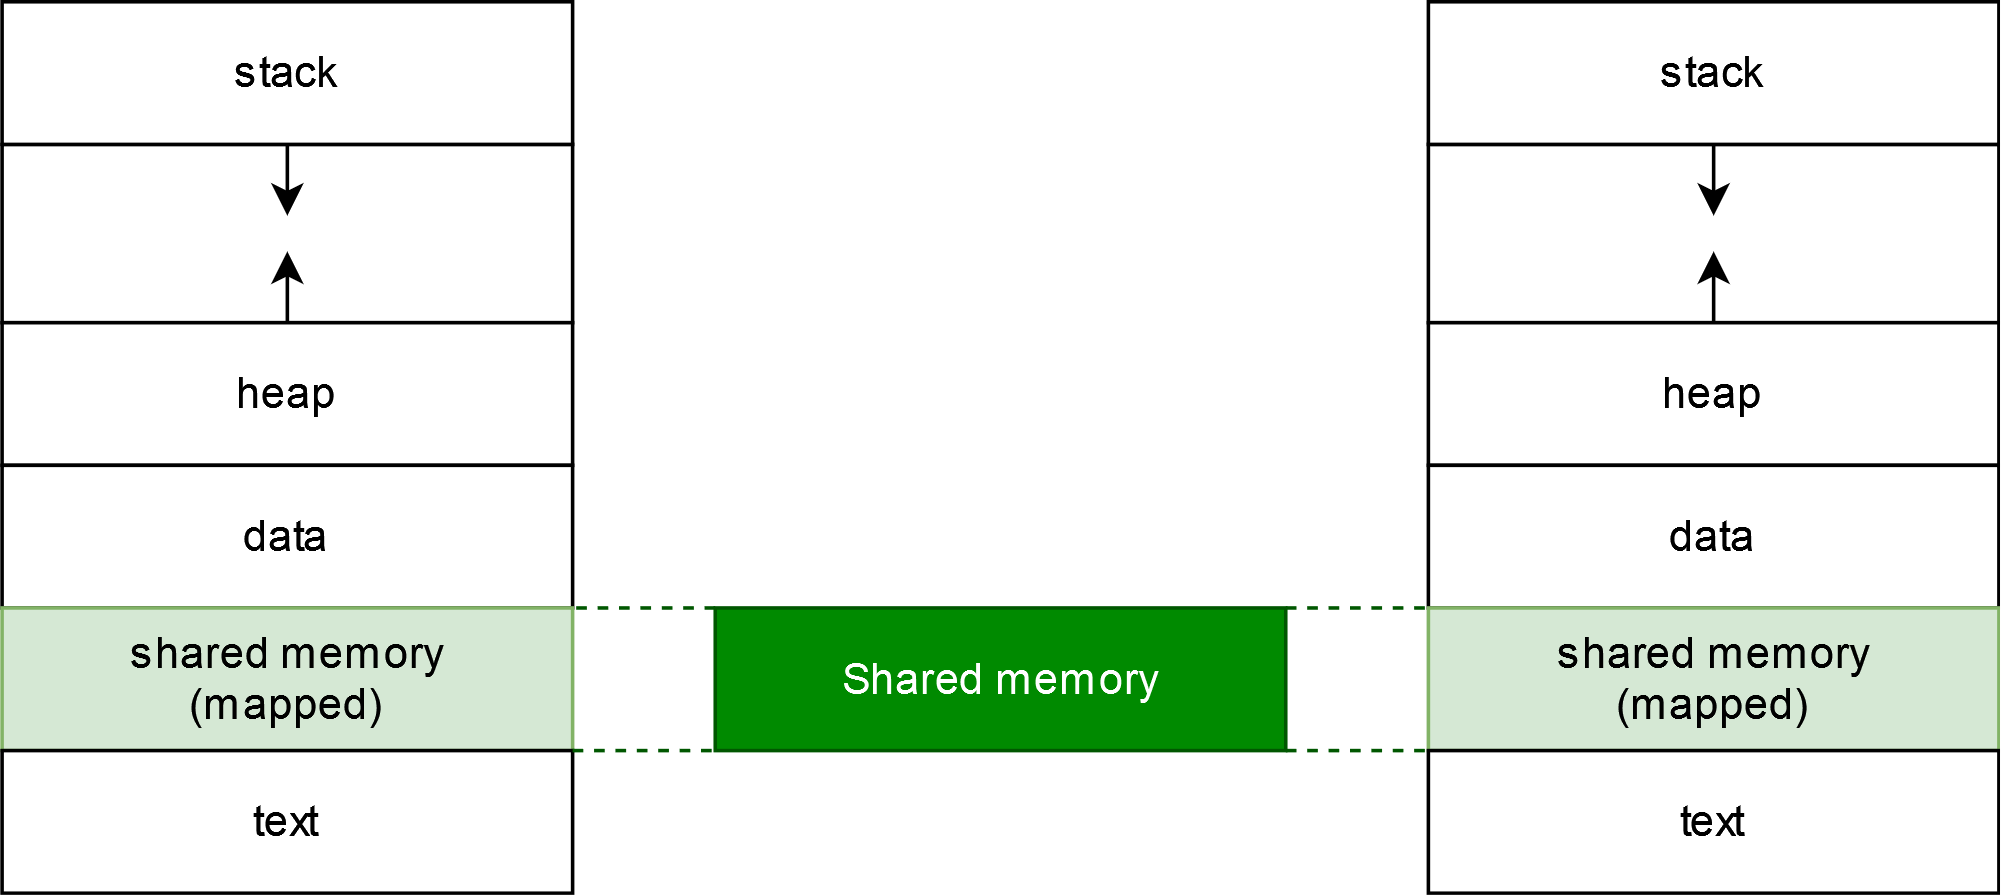
\includegraphics[width=0.75\columnwidth]{figures/shared_memory.png}
	\caption{Schematic address spaces of two processes attached to the same shared memory segment\cite{shared-memory}}
	\label{fig:shared_memory}
\end{figure}

To perform the data transport and initialization of our backend, we used sysV shared memory.
Shared Memory is memory shared between two or more processes which can be read and written by different processes. 
The memory segment is created by the kernel and mapped to the data segments of each attached process as can be seen in \autoref{fig:shared_memory}. 
In comparison to other types of IPC like pipes, shared memory can be accessed directly without needing to copy the data to the processes data segment \cite{unix-programming}.
The attached processes can access shared memory just like normal memory.
SysV shared memory is not synchronized, therefore developers need to implement their own synchronization mechanisms.\cite{unix-programming}.

\begin{figure}[htpb]
	\centering
	\begin{tabular}{c}
		\begin{lstlisting}[language=C]
		int shmget (key_t key, size_t size, int shmflg);
		void *shmat (int shmid, const void *shmaddr, int shmflg);
		int shmdt (const void *shmaddr);
		int shmctl (int shmid, int cmd, struct shmid_ds *buf);
		\end{lstlisting}
	\end{tabular}
	\caption[SysV shmem signatures]{The signatures of the four sysV shared memory calls\cite{unix-programming}}
	\label{fig:sysV-shmem}
\end{figure}

SysV shared memory can be controlled with the four shared memory calls seen in \autoref{fig:sysV-shmem}.
The function \code{shmget()} creates or opens a shared memory segment and returns the corresponding shared memory id on success.
On failure it returns $-1$.
The first argument \code{key} is a unique identifier for the shared memory segment, two calls with the same key will allays try to open the same segment. 
The parameter \code{size} specifies the size of the shared memory segment in bytes.
0 can also be passed if the segment already exists.
The flag \code{shmflg} manages the access privileges: \code{IPC\_CREAT} allows the call to create a new segment, \code{IPC\_EXCL} assures in combination with \code{IPC\_CREAT} that the shared memory segment was created by the process and did not exist previously.
Should the segment allready exist, \code{shmget()} will return -1\cite{unix-programming}.

The second call \code{shmat()} returns a pointer to the shared memory segment with the id \code{shmid}. 
On Failure it returns $-1$.
The second argument \code{shmaddr} tells the kernel where to attach the segment, due to portability reasons it is recommended to pass \code{NULL}.
The last argument \code{shmflg} can be set to \code{SHM\_RDONLY} so the attached process is only able to read, otherwise $0$ is passed\cite{unix-programming}. 
  
To detach an attached shared memory segment the call \code{shmdt()} is used.
The argument \code{shmaddr} is the pointer to the shared memory segment the application wants to detach from.
On success it returns $0$, on failure $-1$\cite{unix-programming}.

The last call \code{shmctl} is used to query or change the status of shared memory segments.
For our purposes the delete functionality is most important.
To delete a shared memory segment with id \code{shmid}, the second argument \code{cmd} must be \code{IPC\_RMID} and \code{buf} must be 0.
The function returns $0$ on success and $-1$ on failure\cite{unix-programming}.


\subsection{SysV Semaphores}

To synchronize our backends shared memory segments we decided to use sysV semaphores.
A semaphore is a data structure which can be used to control the access to a resource.
If a process wants to access the resource he has to check that the semaphores value is positive.
If the semaphores value is positive the process sets the value to $0$ and is able to use the resource after that.
After the process is done using the resource he increments the semaphore to allow other processes to access the resource.

\begin{figure}[htpb]
	\centering
	\begin{tabular}{c}
		\begin{lstlisting}[language=C]
		int semget(key_t key, int n_sems, int flag);
		int semctl(int semid, int sem_num, int command, union semun arg);
		int semop(int semid, struct sembuf *sops, size_t nsops);
		
		struct sembuf {
		unsigned short sem_num;
		short sem_op;
		short sem_flg; };
		\end{lstlisting}
	\end{tabular}
	\caption[SysV semaphores signatures]{The signatures of the three sysV semaphore calls and the definition of the sembuf struct \cite{unix-programming}}
	\label{fig:sysV-semaphores}
\end{figure}

SysV semaphores are managed in semaphore sets which can be controlled with the three calls seen in \autoref{fig:sysV-semaphores}.
To create or open an existing semaphore set \code{semget()} is used.
Parallel to sysV shared memory \code{key} is a unique identifier for the semaphore.
The second argument \code{n\_sems} specifies the number of semaphores in the semaphore set.
The last parameter \code{flag} works like the one for \code{shmget} of sysV shared memory.
The call returns the id of the semaphore set on success and $-1$ on failure\cite{unix-programming}.

The \code{semctl} call is used to control a set of semaphores.
The first argument \code{semid} is used to identify the semaphore set and \code{sem\_num} is used to specify the semaphore value.
The argument \code{command} specifies the action.
For our purposes the most important actions are: \code{SETVAL} which sets the value of a semaphore variable and \code{IPC\_RMID} which deletes the semaphore set.
The union \code{semun} is used as an additional parameter for the commandos.
When using \code{SETVAL}, it specifies the value we want to set the semaphores to.
When using \code{IPC\_RMID}, $0$ can be given as an argument. 
In our usecases the function returns $0$ on success and $-1$ on failure\cite{unix-programming}.

To perform operations on the semaphores the \code{semop()} call is used.
The first argument \code{semctl} identifies the semaphore set.
The second argument \code{sops} points to an array of semaphore operations of type \code{struct sembuf} which specifies the operations to be performed on the semaphore set.
Each \code{sembuf} struct contains \code{sem\_num} to choose the semaphore  from the set, \code{sem\_op} to specify the operation and \code{sem\_flg} to pass extra options.
If \code{sem\_op} is greater than 0, the semaphore gets freed, if its is less than zero it gets locked and if it is equal to zero the call immediately returns. 
The call waits until he can access the semaphore or if the flag \code{IPC\_NOWAIT} is set it returns an error if it can not immediately access the semaphore.  
The flag \code{SEM\_UNDO} ensures that an accessed semaphore gets reset if the process should terminate prematurely. 
The last parameter \code{nsops} is the length of the \code{sops} array\cite{unix-programming}.